\documentclass{beamer}

\usepackage[utf8]{inputenc}
\usepackage[spanish]{babel}
\usepackage{amsmath}
\usepackage[nosetup]{evan}
\usetheme{Madrid}
%\usetheme{Goddard}
\hypersetup{colorlinks,allcolors=.,urlcolor=magenta}
\usepackage[table]{xcolor} % Para definir colores en tablas
\usepackage{graphicx} % Para redimensionar la tabla
\usepackage{multicol}

\title{Investigación de Operaciones I}
\subtitle{Unidad 2: Aspectos de Dualidad y Análisis de Sensibilidad}
\author[Ricardo Largaespada]{Ricardo Jesús Largaespada Fernández}
\institute[UNI]{Ingeniería de Sistemas, DACTIC, UNI}
\date{15 de Octubre, 2024}

\begin{document}

\frame{\titlepage}

\begin{frame}
\frametitle{Agenda}
\tableofcontents
\end{frame}

\begin{frame}
\frametitle{Contenidos}
\begin{itemize}
\item Método Dual Simplex.
\begin{itemize}
\item Introducción al Análisis gráfico sensibilidad.
\end{itemize}
\item Análisis Post óptimo de Sensibilidad.
\begin{itemize}
\item Cambios que afectan la factibilidad
\item Cambio en los lados derechos
\item Rango de Factibilidad
\item Adición de Nuevas Restricciones
\end{itemize}
\end{itemize}

\pause
\textbf{Objetivos de Aprendizaje}
    \begin{enumerate}
        \item Analizar cómo los cambios en los coeficientes de la función objetivo, el rango de optimalidad y la adición de una nueva variable afectan la optimalidad de un problema de programación lineal y cómo realizar un análisis post óptimo de sensibilidad en estos casos.
    \end{enumerate}
\end{frame}

\begin{frame}{Un ejemplo motivador}
Una empresa vende dos productos.
\begin{itemize}
    \item Producir una unidad del producto 1 requiere 1 unidad del recurso 1 y 1 unidad del recurso 2.
    \item Producir una unidad del producto 2 requiere 1 unidad del recurso 1 y 2 unidades del recurso 2.
    \item Cada unidad de los productos 1 y 2 se puede vender a \$2 y \$3, respectivamente.
    \item La cantidad total de los recursos 1 y 2 disponibles es de 4 y 6 unidades, respectivamente.
\end{itemize}
Encuentra un plan de producción óptimo que maximice los ingresos totales por ventas.

\textbf{Formulación del Programa Lineal:}
\begin{align*}
\max \quad 2x_1 + 3x_2\\
\text{s.a.:} \quad x_1 + x_2 \leq 4\\
x_1 + 2x_2 \leq 6\\
x_1, x_2 \geq 0
\end{align*}

\end{frame}

\begin{frame}{Un ejemplo motivador}
\begin{columns}
\begin{column}{0.6\linewidth}

    \begin{itemize}
        \item Podemos usar el método simplex para resolverlo:
    \end{itemize}
    
    \[
    \begin{array}{cccc|c}
        -2 & -3 & 0 & 0 & 0 \\
        \hline
        \fbox{1} & 1 & 1 & 0 & 4 \\
        1 & 2 & 0 & 1 & 6 
    \end{array}
    \quad \rightarrow \quad
    \begin{array}{cccc|c}
        0 & -1 & 2 & 0 & 8 \\
        \hline
        1 & 1 & 1 & 0 & 4 \\
        0 & \fbox{1} & -1 & 1 & 2 
    \end{array}
    \]

    \[
    \begin{array}{cccc|c}
        0 & 0 & 1 & 1 & 10 \\
        \hline
        1 & 0 & 2 & -1 & 2 \\
        0 & 1 & -1 & 1 & 2 
    \end{array}
    \]

    \vspace{0.3cm}

    \begin{itemize}
        \item Una solución óptima es \( (x_1^*, x_2^*) = (2, 2) \). El valor del objetivo es \( z^* = 10 \).
    \end{itemize}
\end{column}
\begin{column}{0.4\linewidth}
    \begin{figure}[h]
        \centering
        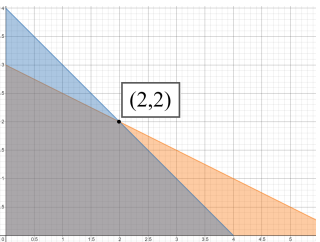
\includegraphics[width=0.4\textwidth]{images/simplex_dual1.png}
        \caption{Representación gráfica de la solución óptima.}
    \end{figure}
\end{column}
\end{columns}
\end{frame}

\begin{frame}{Una nueva actividad}
    \begin{itemize}
        \item Supongamos que ahora la empresa puede producir un tercer producto.
        \item Una unidad del producto 3 requiere solo 1 unidad del recurso 2 y puede venderse a 8.
        \item La nueva formulación del Programa Lineal es:
    \end{itemize}
    
    \[
    \max \quad 2x_1 + 3x_2 + 8x_3
    \]
    
    \[
    \text{s.a.:} \quad 
    \begin{aligned}
    x_1 + x_2 &\leq 4 \\
    x_1 + 2x_2 + x_3 &\leq 6 \\
    x_1, x_2, x_3 &\geq 0
    \end{aligned}
    \]
    
    \vspace{0.5cm}
    
    \begin{itemize}
        \item ¿Podemos encontrar un plan óptimo?
    \end{itemize}
\end{frame}

\begin{frame}{Una nueva actividad}
    \begin{itemize}
        \item Siempre podemos resolver el nuevo programa lineal desde cero:
    \end{itemize}
    \[
    \begin{array}{ccccc|c}
        -2 & -3 & -8 & 0 & 0 & 0 \\
        \hline
        1 & 1 & 0 & 1 & 0 & 4 \\
        1 & 2 & \fbox{1} & 0 & 1 & 6 
    \end{array}
    \quad \rightarrow \quad
    \begin{array}{ccccc|c}
        6 & 13 & 0 & 0 & 8 & 48 \\
        \hline
        1 & 1 & 0 & 1 & 0 & 4 \\
        1 & 2 & 1 & 0 & 1 & 6 
    \end{array}
    \]
    \begin{itemize}
        \item Una solución óptima es \( (x_1, x_2, x_3) = (0, 0, 6) \) con \( z = 48 \).
    \end{itemize}
\end{frame}

\begin{frame}{¿Podemos hacerlo mejor?}
    \begin{itemize}
        \item ¿Realmente necesitamos resolver el nuevo problema desde cero?
        \begin{itemize}
            \item Acabamos de resolver un problema con \(n\) actividades y obtuvimos una solución óptima.
            \item El nuevo problema tiene \(n + 1\) actividades. Las \(n\) actividades originales permanecen sin cambios. Los recursos permanecen sin cambios.
            \item ¡El nuevo problema es muy similar al problema original!
            \item ¿Podemos partir de una solución óptima del problema original en lugar de comenzar desde el principio? ¡Eso puede ahorrar mucho tiempo!
        \end{itemize}
        
        \item Si la factibilidad del problema original es una duda (es decir, si se necesita una implementación en dos fases), ¡la diferencia se hace más evidente!
    \end{itemize}
\end{frame}

\begin{frame}{¿Podemos hacerlo mejor?}
    \begin{itemize}
        \item ¡La respuesta es definitivamente sí!
        
        \item Cuando el conjunto de variables de decisión cambia de \( (x_1, x_2) \) a \( (x_1, x_2, x_3) \), la solución \( (x_1^*, x_2^*, 0) \) es ciertamente factible para el nuevo problema.
        \begin{itemize}
            \item Es como eliminar la nueva columna agregada en el problema.
            \item Simplemente ignoramos la nueva opción.
        \end{itemize}
        
        \item Todo lo que necesitamos hacer es verificar si debemos producir el producto 3.
        \begin{itemize}
            \item Si no, la solución actual \( (x_1^*, x_2^*, 0) \) es óptima.
            \item Si sí, aumentamos la variable no básica \( x_3 \) hasta que una variable básica se vuelva 0.
        \end{itemize}
        
        \item ¿Cómo determinamos esto?
        \begin{itemize}
            \item ¡Todo lo que necesitamos es el costo reducido de \(x_3\)!
        \end{itemize}
    \end{itemize}
\end{frame}

\begin{frame}{Evaluando la nueva actividad}
    \begin{itemize}
        \item Ahora estamos listos para evaluar la nueva actividad (producto 3).
    \end{itemize}

    \vspace{0.3cm}

    \textbf{Nuestro problema original:}
    \[
    \max \quad 2x_1 + 3x_2
    \]
    \[
    \text{s.a.:} \quad 
    \begin{aligned}
    x_1 + x_2 &\leq 4 \\
    x_1 + 2x_2 &\leq 6 \\
    x_1, x_2 &\geq 0
    \end{aligned}
    \]

    \textbf{Nuestro nuevo problema:}
    \[
    \max \quad 2x_1 + 3x_2 + 8x_3
    \]
    \[
    \text{s.a.:} \quad 
    \begin{aligned}
    x_1 + x_2 &\leq 4 \\
    x_1 + 2x_2 + x_3 &\leq 6 \\
    x_1, x_2, x_3 &\geq 0
    \end{aligned}
    \]
\end{frame}

\begin{frame}{Evaluando la nueva actividad}
    \begin{columns}
        \column{0.5\textwidth}
        \begin{itemize}
            \item Recordemos que tenemos el cuadro óptimo para el problema original:
        \end{itemize}

        \[
        \begin{array}{cccc|c}
            0 & 0 & 1 & 1 & 10 \\
            \hline
            1 & 0 & 2 & -1 & 2 \\
            0 & 1 & -1 & 1 & 2
        \end{array}
        \]
        \[
        \underbrace{\text{básica}}_{\phantom{a}} \quad
        \underbrace{\text{no básica}}
        \]

        \column{0.5\textwidth}
        \begin{itemize}
            \item El cuadro inicial para el nuevo problema debería tener solo una columna faltante:
        \end{itemize}

        \[
        \begin{array}{ccccc|c}
            0 & 0 & ? & 1 & 1 & 10 \\
            \hline
            1 & 0 & ? & 2 & -1 & 2 \\
            0 & 1 & ? & -1 & 1 & 2
        \end{array}
        \]
        \[
        \underbrace{\text{básica}}_{\phantom{a}} \quad
        \underbrace{\text{no básica}}
        \]
    \end{columns}
        \begin{itemize}
        \item Vamos a calcular los valores en esa columna.
        \item El vector de coeficientes de restricción para las variables no básicas es \( A_B^{-1} A_N \).
\end{itemize}
\end{frame}

\begin{frame}{Evaluando la nueva actividad}
\begin{itemize}
        \begin{itemize}
            \item Para la columna \( j \), esa columna es \( A_B^{-1} A_j \).
            \item En nuestro ejemplo, es:
        \end{itemize}
        \[
        \begin{bmatrix}
            2 & -1 \\
            -1 & 1
        \end{bmatrix}
        \begin{bmatrix}
            0 \\
            1
        \end{bmatrix}
        =
        \begin{bmatrix}
            -1 \\
            1
        \end{bmatrix}.
        \]
        
        \item El vector de costos reducidos para las variables no básicas es \( c_B^T A_B^{-1} A_N - c_N^T \).
        \begin{itemize}
            \item Para la columna \( j \), ese valor es \( c_B^T A_B^{-1} A_j - c_j \).
            \item En nuestro ejemplo, es:
        \end{itemize}
        \[
        \begin{bmatrix}
            2 & 3
        \end{bmatrix}
        \begin{bmatrix}
            -1 \\
            1
        \end{bmatrix}
        - 8 = -7.
        \]
    \end{itemize}
    
    \begin{columns}
        \column{0.5\textwidth}
        \[
        \begin{array}{ccccc|c}
            0 & 0 & ? & 1 & 1 & 10 \\
            \hline
            1 & 0 & ? & 2 & -1 & 2 \\
            0 & 1 & ? & -1 & 1 & 2
        \end{array}
        \]
        \[
        \underbrace{\text{básica}}_{\phantom{a}} \quad
        \underbrace{\text{no básica}}
        \]

        \column{0.5\textwidth}
        \[
        \begin{array}{ccccc|c}
            0 & 0 & -7 & 1 & 1 & 10 \\
            \hline
            1 & 0 & -1 & 2 & -1 & 2 \\
            0 & 1 & 1 & -1 & 1 & 2
        \end{array}
        \]
        \[
        \underbrace{\text{básica}}_{\phantom{a}} \quad
        \underbrace{\text{no básica}}
        \]
    \end{columns}
\end{frame}

\begin{frame}{Evaluando la nueva actividad}
    \begin{itemize}
        \item Partamos del cuadro inicial para el nuevo problema:
    \end{itemize}
    {\tiny
    \[
    \begin{array}{ccccc|c}
        0 & 0 & -7 & 1 & 1 & 10 \\
        \hline
        1 & 0 & -1 & 2 & -1 & 2 \\
        0 & 1 & 1 & -1 & 1 & 2
    \end{array}
    \quad \rightarrow \quad
    \begin{array}{ccccc|c}
        0 & 7 & 0 & -6 & 8 & 24 \\
        \hline
        1 & 1 & 0 & 1 & 0 & 4 \\
        0 & 1 & 1 & -1 & 1 & 2
    \end{array}
    \quad \rightarrow \quad
    \begin{array}{ccccc|c}
        6 & 13 & 0 & 0 & 8 & 48 \\
        \hline
        1 & 1 & 0 & 1 & 0 & 4 \\
        1 & 2 & 1 & 0 & 1 & 6
    \end{array}
    \]
    }
    \begin{itemize}
        \item Una solución óptima es \( (x_1, x_2, x_3) = (0, 0, 6) \) con \( z^{**} = 48 \).
        \item Esto es exactamente como omitir las primeras iteraciones desde el principio hasta el cuadro inicial.
        \begin{itemize}
            \item Así se ahorra tiempo.
        \end{itemize}
        \item Podemos acelerar aún más usando la representación matricial.
        \begin{itemize}
            \item No es necesario trabajar con el cuadro completo.
        \end{itemize}
    \end{itemize}
\end{frame}

\begin{frame}{Una nueva restricción}
\begin{columns}
\begin{column}{0.5\textwidth}
    \begin{itemize}
        \item Recordemos nuestro ejemplo:
    \end{itemize}

    \[
    \max \quad 2x_1 + 3x_2
    \]
    \[
    \text{s.a.:} \quad 
    \begin{aligned}
        x_1 + x_2 &\leq 4 \\
        x_1 + 2x_2 &\leq 6 \\
        x_1, x_2 &\geq 0
    \end{aligned}
    \]

    \begin{itemize}
        \item Sabemos cómo evaluar una nueva actividad.
    \end{itemize}
    \end{column}
    \begin{column}{0.5\textwidth}
    \begin{itemize}
        \item ¿Qué sucede si ahora tenemos una nueva restricción? Por ejemplo:
    \end{itemize}
    \[
    \max \quad 2x_1 + 3x_2
    \]
    \[
    \text{s.a.:} \quad 
    \begin{aligned}
        x_1 + x_2 &\leq 4 \\
        x_1 + 2x_2 &\leq 6 \\
        x_1 &\leq 1 \\
        x_1, x_2 &\geq 0
    \end{aligned}
    \] 
    \end{column}
    \end{columns}
\end{frame}

\begin{frame}{Una nueva restricción}
    \begin{itemize}
        \item Intuitivamente, podemos probar la solución óptima original \( (x_1^*, x_2^*) = (2, 2) \) en la nueva restricción.
        \begin{itemize}
            \item Si es factible, es óptima para el nuevo problema.
            \item En nuestro ejemplo, no es factible porque \( 2 > 1 \).
            \item ¿Qué sucede si no es factible?
        \end{itemize}
        
        \item Veamos el cuadro (tableau) para obtener más ideas.
    \end{itemize}
\end{frame}

\begin{frame}{El nuevo tableau con la nueva restricción}
    \begin{itemize}
        \item Recordemos nuestro tableau óptimo original:
    \end{itemize}

    \[
    \begin{array}{cccc|c}
        0 & 0 & 1 & 1 & 10 \\
        \hline
        1 & 0 & 2 & -1 & 2 \\
        0 & 1 & -1 & 1 & 2
    \end{array}
    \]

    \begin{itemize}
        \item Con una nueva restricción \(x_1 \leq 1\) (que también introduce una nueva variable de holgura \(s_3\)), ¿cómo debería ser el nuevo tableau?
        \item Nuevamente, nos basamos en la representación matricial.
    \end{itemize}
\end{frame}

\begin{frame}{El nuevo tableau con la nueva restricción}
    \begin{itemize}
        \item Incluyamos \( s_3 \) como una variable básica (ya que se viola la nueva restricción).
        \item Sea \( B = (x_1, x_2, s_3) \) y \( N = (s_1, s_2) \).
    \end{itemize}

    \[
    \mathbf{c_B} = 
    \begin{bmatrix}
        2 \\ 3 \\ 0
    \end{bmatrix}, \quad
    \mathbf{c_N} = 
    \begin{bmatrix}
        0 \\ 0
    \end{bmatrix}, \quad
    A_B = 
    \begin{bmatrix}
        1 & 1 & 0 \\
        1 & 2 & 0 \\
        1 & 0 & 1
    \end{bmatrix},
    \]
    
    \[
    A_N = 
    \begin{bmatrix}
        1 & 0 \\
        0 & 1 \\
        0 & 0
    \end{bmatrix}, \quad
    \mathbf{b} = 
    \begin{bmatrix}
        4 \\ 6 \\ 1
    \end{bmatrix}.
    \]

    \begin{itemize}
        \item Entonces tenemos \( A_B^{-1} = 
        \begin{bmatrix}
            2 & -1 & 0 \\
            -1 & 1 & 0 \\
            -2 & 1 & 1
        \end{bmatrix} \), \quad
        \( A_B^{-1} A_N = 
        \begin{bmatrix}
            2 & -1 \\
            -1 & 1 \\
            -2 & 1
        \end{bmatrix} \).
    \end{itemize}

    \[
    A_B^{-1} \mathbf{b} = 
    \begin{bmatrix}
        2 \\ 2 \\ -1
    \end{bmatrix}, \quad
    \mathbf{c_B}^T A_B^{-1} A_N - \mathbf{c_N}^T = 
    \begin{bmatrix}
        1 & 1
    \end{bmatrix}, \quad
    \mathbf{c_B}^T A_B^{-1} \mathbf{b} = 10.
    \]
\end{frame}

\begin{frame}{El nuevo tableau con la nueva restricción}
    \begin{itemize}
        \item Esto nos da un nuevo tableau:
    \end{itemize}

    \[
    \begin{array}{ccccc|c}
        0 & 0 & 1 & 1 & 0 & 10 \\
        \hline
        1 & 0 & 2 & -1 & 0 & 2 \\
        0 & 1 & -1 & 1 & 0 & 2 \\
        0 & 0 & -2 & 1 & 1 & -1
    \end{array}
    \]

    \[
    \underbrace{\text{básica}}_{\phantom{a}} \quad \underbrace{\text{NB}} \quad \underbrace{\text{básica}}_{\phantom{a}}
    \]
\end{frame}

\begin{frame}{Una base no factible}
    \begin{itemize}
        \item El tableau:
    \end{itemize}

    \[
    \begin{array}{ccccc|c}
        0 & 0 & 1 & 1 & 0 & 10 \\
        \hline
        1 & 0 & 2 & -1 & 0 & 2 \\
        0 & 1 & -1 & 1 & 0 & 2 \\
        0 & 0 & -2 & 1 & 1 & -1
    \end{array}
    \]

    \begin{itemize}
        \item Este es un tableau simplex no válido: su columna del lado derecho contiene un valor negativo.
        \begin{itemize}
            \item En otras palabras, \( B = (x_1, x_2, s_3) \) no es factible, como ya sabemos.
        \end{itemize}

        \item ¿Qué deberíamos hacer?
    \end{itemize}
\end{frame}

\begin{frame}{Dualidad en Programación Lineal}
    \begin{itemize}
        \item Recordemos que sabemos cómo manejar una nueva variable.
        \begin{itemize}
            \item Evaluamos su costo reducido.
            \item Ejecutamos algunas iteraciones del método simplex si es necesario.
        \end{itemize}

        \item No sabemos cómo manejar una nueva restricción.
        \begin{itemize}
            \item No sabemos cómo ejecutar iteraciones del método simplex para esto.
        \end{itemize}

        \item Pero espera... conocemos la dualidad en programación lineal.
        \begin{itemize}
            \item Sabemos que una restricción en el problema primal es una variable dual.
            \item Si un problema primal tiene una nueva restricción, su dual tendrá una nueva variable.
            \item ¡Sabemos cómo manejar el problema dual!
        \end{itemize}
    \end{itemize}
\end{frame}

\begin{frame}{Dualidad en Programación Lineal}
    \begin{itemize}
        \item Nuestro problema primal original es:
    \end{itemize}

    \[
    \max \quad 2x_1 + 3x_2
    \]
    \[
    \text{s.a.:} \quad
    \begin{aligned}
        x_1 + x_2 &\leq 4 \\
        x_1 + 2x_2 &\leq 6 \\
        x_1, x_2 &\geq 0
    \end{aligned}
    \]

    \vspace{0.5cm}

    \begin{itemize}
        \item Nuestro problema dual original es:
    \end{itemize}

    \[
    \min \quad 4y_1 + 6y_2
    \]
    \[
    \text{s.a.:} \quad
    \begin{aligned}
        y_1 + y_2 &\geq 2 \\
        y_1 + 2y_2 &\geq 3 \\
        y_1, y_2 &\geq 0
    \end{aligned}
    \]
\end{frame}

\begin{frame}{Dualidad en Programación Lineal}
    \begin{itemize}
        \item Nuestro problema primal con una nueva restricción es:
    \end{itemize}

    \[
    \max \quad 2x_1 + 3x_2
    \]
    \[
    \text{s.a.:} \quad
    \begin{aligned}
        x_1 + x_2 &\leq 4 \\
        x_1 + 2x_2 &\leq 6 \\
        x_1 &\leq 1 \\
        x_1, x_2 &\geq 0
    \end{aligned}
    \]

    \vspace{0.5cm}

    \begin{itemize}
        \item Nuestro problema dual con una nueva variable es:
    \end{itemize}

    \[
    \min \quad 4y_1 + 6y_2 + y_3
    \]
    \[
    \text{s.a.:} \quad
    \begin{aligned}
        y_1 + y_2 + y_3 &\geq 2 \\
        y_1 + 2y_2 &\geq 3 \\
        y_1, y_2, y_3 &\geq 0
    \end{aligned}
    \]

    \begin{itemize}
        \item La solución óptima del dual original no es óptima para el nuevo dual.
        \item Podemos resolver el nuevo dual para resolver el nuevo primal.
    \end{itemize}
\end{frame}

\begin{frame}{El método dual simplex}
    \begin{itemize}
        \item Aunque entendemos la idea, realmente no necesitamos trabajar en el problema dual.
        \item Podemos utilizar el \textit{método dual simplex} directamente.
        \item El método simplex (primal) para un problema de maximización:
        \begin{itemize}
            \item Buscar un \textbf{costo reducido negativo} para una variable entrante.
            \item Realizar la prueba de razón para encontrar un valor en el lado derecho (RHS) que llegue a 0 primero para una variable saliente.
            \item Mantenemos la factibilidad primal y corregimos la no factibilidad dual.
        \end{itemize}
        \item El método dual simplex para un problema de maximización:
        \begin{itemize}
            \item Buscar un \textbf{valor negativo en el lado derecho (RHS)} para una variable saliente.
            \item Realizar la prueba de razón para encontrar un \textbf{costo reducido que llegue a 0 primero} para una variable entrante.
            \item Mantenemos la factibilidad dual y corregimos la no factibilidad primal.
        \end{itemize}
    \end{itemize}
\end{frame}

\begin{frame}{Un ejemplo}
    \begin{itemize}
        \item Recordemos nuestro nuevo problema primal y su tableau no válido:
    \end{itemize}
\begin{columns}
    \begin{column}{0.5\textwidth}
    \[
    \max \quad 2x_1 + 3x_2
    \]
    \[
    \text{s.a.:} \quad
    \begin{aligned}
        x_1 + x_2 &\leq 4 \\
        x_1 + 2x_2 &\leq 6 \\
        x_1 &\leq 1 \\
        x_1, x_2 &\geq 0
    \end{aligned}
    \]        
    \end{column}
    \begin{column}{0.5\textwidth}
    \[
    \begin{array}{ccccc|c}
        0 & 0 & 1 & 1 & 0 & 10 \\
        \hline
        1 & 0 & 2 & -1 & 0 & 2 \\
        0 & 1 & -1 & 1 & 0 & 2 \\
        0 & 0 & -2 & 1 & 1 & -1
    \end{array}
    \]        
    \end{column}

\end{columns}

    \begin{itemize}
        \item Busquemos un \textbf{valor negativo en el lado derecho (RHS)} para una variable saliente:
        \begin{itemize}
            \item \( s_3 \) debería ser la variable saliente.
        \end{itemize}

        \item ¿Dónde está el pivote?
        \begin{itemize}
            \item Necesitamos corregir la no factibilidad primal haciendo que \(-1\) sea no negativo.
            \item El pivote debe ser \textbf{negativo} para que una operación por filas realice la corrección.
        \end{itemize}
    \end{itemize}
\end{frame}

\begin{frame}{Pivoteo}
    \[
    \begin{array}{ccccc|c}
        0 & 0 & 1 & 1 & 0 & 10 \\
        \hline
        1 & 0 & 2 & -1 & 0 & 2 \\
        0 & 1 & -1 & 1 & 0 & 2 \\
        0 & 0 & -2 & 1 & 1 & -1
    \end{array}
    \quad \xrightarrow{\text{oper. fila 3}} \quad
    \begin{array}{ccccc|c}
        0 & 0 & 1 & 1 & 0 & 10 \\
        \hline
        1 & 0 & 2 & -1 & 0 & 2 \\
        0 & 1 & -1 & 1 & 0 & 2 \\
        0 & 0 & 1 & -\frac{1}{2} & -\frac{1}{2} & \frac{1}{2}
    \end{array}
    \]

    \vspace{0.5cm}

    \[
    \xrightarrow{\text{operación por filas en las filas 0, 1 y 2}} \quad
    \begin{array}{ccccc|c}
        0 & 0 & 0 & \frac{3}{2} & \frac{1}{2} & \frac{19}{2} \\
        \hline
        1 & 0 & 0 & 0 & 1 & 1 \\
        0 & 1 & 0 & \frac{1}{2} & -\frac{1}{2} & \frac{5}{2} \\
        0 & 0 & 1 & -\frac{1}{2} & -\frac{1}{2} & \frac{1}{2}
    \end{array}
    \]
\end{frame}

\begin{frame}{Pivoteo}
    \begin{itemize}
        \item Después de una iteración, obtenemos:
    \end{itemize}

    \[
    \begin{array}{ccccc|c}
        0 & 0 & 0 & \frac{3}{2} & \frac{1}{2} & \frac{19}{2} \\
        \hline
        1 & 0 & 0 & 0 & 1 & 1 \\
        0 & 1 & 0 & \frac{1}{2} & -\frac{1}{2} & \frac{5}{2} \\
        0 & 0 & 1 & -\frac{1}{2} & -\frac{1}{2} & \frac{1}{2}
    \end{array}
    \]

    \begin{itemize}
        \item \( s_3 \) sale y \( s_1 \) entra.
        \item La solución básica actual es \( (x_1, x_2, s_1, s_2, s_3) = \left(1, \frac{5}{2}, \frac{1}{2}, 0, 0\right) \). Es factible.
        \item Corresponde a la solución \( (x_1, x_2) = \left(1, \frac{5}{2}\right) \) con \( z = \frac{19}{2} \). Es óptima.
    \end{itemize}
\end{frame}

\begin{frame}{Otro ejemplo (puramente pedagógico)}
    \begin{itemize}
        \item ¿Qué pasa si tenemos \textbf{múltiples valores negativos en el RHS}? Por ejemplo:
    \end{itemize}

    \[
    \begin{array}{ccccc|c}
        0 & 0 & 1 & 1 & 0 & 10 \\
        \hline
        1 & 0 & -2 & -1 & 0 & -2 \\
        0 & 1 & -1 & 1 & 0 & 2 \\
        0 & 0 & -2 & 1 & 1 & -1
    \end{array}
    \]

    \begin{itemize}
        \item En este caso, puedes elegir cualquiera.
        \item Por ejemplo, si adoptamos la regla del índice más pequeño, elegiremos \(x_1\).
    \end{itemize}

    \begin{itemize}
        \item ¿Qué pasa si tenemos \textbf{múltiples números negativos en esa fila}?
        \begin{itemize}
            \item Necesitamos mantener la factibilidad dual (hacer que los costos reducidos sean no negativos).
            \item Una prueba de razón nos ayudará a elegir uno (¿cuál?).
        \end{itemize}
    \end{itemize}
\end{frame}

\begin{frame}{Otro ejemplo (puramente pedagógico)}
    \begin{itemize}
        \item Pivotear en \(-2\) es bueno (y \( \left|\frac{1}{-2}\right| < \left|\frac{1}{-1}\right| \)):
    \end{itemize}

    \[
    \begin{array}{ccccc|c}
        0 & 0 & 1 & 1 & 0 & 10 \\
        \hline
        1 & 0 & -2 & -1 & 0 & -2 \\
        0 & 1 & -1 & 1 & 0 & 2 \\
        0 & 0 & -2 & 1 & 1 & -1
    \end{array}
    \quad \rightarrow \quad
    \begin{array}{ccccc|c}
        \frac{1}{2} & 0 & 0 & \frac{1}{2} & 0 & 9 \\
        \hline
        -\frac{1}{2} & 0 & 1 & \frac{1}{2} & 0 & 1 \\
        -\frac{1}{2} & 1 & 0 & \frac{3}{2} & 0 & 3 \\
        -1 & 0 & 0 & 2 & 1 & 1
    \end{array}
    \]

    \vspace{0.5cm}

    \begin{itemize}
        \item Pivotear en \(-1\) es malo (y \( \left|\frac{1}{-1}\right| > \left|\frac{1}{-2}\right| \)):
    \end{itemize}

    \[
    \begin{array}{ccccc|c}
        0 & 0 & 1 & 1 & 0 & 10 \\
        \hline
        1 & 0 & -2 & -1 & 0 & -2 \\
        0 & 1 & -1 & 1 & 0 & 2 \\
        0 & 0 & -2 & 1 & 1 & -1
    \end{array}
    \quad \rightarrow \quad
    \begin{array}{ccccc|c}
        1 & 0 & -1 & 0 & 0 & 8 \\
        \hline
        -1 & 0 & 2 & 1 & 0 & 2 \\
        1 & 1 & -3 & 0 & 0 & 0 \\
        -1 & 0 & -4 & 1 & 1 & -3
    \end{array}
    \]
\end{frame}

\begin{frame}{Observaciones}
    \begin{itemize}
        \item El método dual simplex nos ayuda a manejar restricciones adicionales.
        \item La \textbf{regla de pivoteo}:
        \begin{itemize}
            \item \textbf{Salida}: Una variable básica que es negativa (una fila con un RHS negativo).
            \item \textbf{Prueba de razón}: Para aquellas columnas no básicas con elementos negativos en la fila de salida, se toman los costos reducidos como numeradores y los valores absolutos de los elementos negativos como denominadores.
            \item \textbf{Entrada}: Una variable no básica (una columna) con la razón más pequeña.
        \end{itemize}

        \item Se usa en muchas situaciones, por ejemplo:
        \begin{itemize}
            \item Cuando usamos \textit{branch and bound} para resolver un programa entero, seguimos agregando restricciones a los nodos existentes.
            \item Para resolver un nuevo nodo con una restricción adicional, el método dual simplex es de gran ayuda.
        \end{itemize}
    \end{itemize}
\end{frame}

\end{document}
